\documentclass[a4paper, 12pt, oneside, titlepage, openany]{book}

\usepackage{titlesec} %Para el seccionado, debe colocarse al principio este package.

%Interlineado de todo el documento a 1.5
\usepackage{setspace}
%\spacing{1.5} ir\'a en diferentes secciones

\usepackage{color,soulutf8}
\usepackage{float}
\floatstyle{boxed}
\restylefloat{table}
\restylefloat{figure}
\usepackage[section,above,below]{placeins}
\usepackage{microtype}
\usepackage{amsmath,amsfonts,amssymb}
\allowdisplaybreaks
\usepackage{stmaryrd}
\SetSymbolFont{stmry}{bold}{U}{stmry}{m}{n}
\usepackage[braket]{qcircuit}
\usepackage{proof}
\usepackage{tikz}
\usepackage{multicol,multirow}
\usepackage{graphicx}
\usepackage{array,longtable}
\usepackage{wrapfig}
\usepackage{commath}
\usepackage{MnSymbol}
\usepackage{anyfontsize} % permite tamaño de fuentes arbitrarios
\usepackage{tikz, pgfplots}
\pgfplotsset{compat=newest}
\usepackage{hyperref}

\usepackage{physics} %Para las derivadas

\usepackage{pdfpages}

% automatic math mode, centered
\newcolumntype{C}{>{$}c<{$}}
\newcolumntype{R}{>{$}r<{$}}
\newcolumntype{L}{>{$}l<{$}}

\usepackage{mleftright} %Para un mejor ajuste en los logaritmos
\newcommand{\lnn}[1]{
  \ln\left(#1\right)
}

\newcommand{\lnb}[1]{
  \ln\mleft(#1\mright)
}

\newtheorem{theorem}{Teorema}[section]
\newtheorem{lemma}[theorem]{Lema}
\newtheorem{corollary}[theorem]{Colorario}
\newtheorem{proposition}[theorem]{Proposicion}

\newenvironment{definition}[1][Definici\'on]{\begin{trivlist}
%Como en el libro de Tromba, an\'alisis Matem\'atico. En negrita y sin enumeraci\'on:
\item[\hskip \labelsep {\bfseries #1}]}{\end{trivlist}} 
\newenvironment{exercise}[1][Ejercicio]{\begin{trivlist}
\item[\hskip \labelsep {\bfseries #1}]}{\end{trivlist}} 
\newenvironment{proof}[1][Demostraci\'on]{\begin{trivlist}
\item[\hskip \labelsep {\itshape #1}]}{\end{trivlist}}
\newenvironment{example}[1][Ejemplo]{\begin{trivlist}
\item[\hskip \labelsep {\itshape #1}]}{\end{trivlist}}
\newenvironment{remark}[1][Comentario]{\begin{trivlist}
\item[\hskip \labelsep {\itshape #1}]}{\end{trivlist}}

\usepackage{lastpage}
\usepackage{titleps}

\newpagestyle{ruled}
%En los tres corchetes, para izq, centro, der, paginas pares. En llaves, paginas impares.
%Solo llaves es para ambas paginas.
	{   
   %\sethead{
\includegraphics[width=3.7cm]{../images/UBA_LARGE}}{\Title}{\Author}\headrule
	\sethead{
\includegraphics[width=3.7cm]{../images/UBA_LARGE}}
			{\parbox[b]{0.43\textwidth}{\centering F\'isica 1}} %b es para poner texto sobre el bottom
			{Nicolás Alberto Monzón}\headrule
	\setfoot[][][P\'agina \thepage\ de \pageref{LastPage}]{}{}{P\'agina \thepage\ de \pageref{LastPage}}\footrule
	}
	\pagestyle{ruled}
%Cambiar el color de la linea divisora:
%\renewcommand\makeheadrule{\color{cyan}\rule[-.3\baselineskip]{\linewidth}{0.4pt}}
%\renewcommand\makefootrule{\color{cyan}\rule[\baselineskip]{\linewidth}{0.4pt}}

%M\'argenes
\usepackage{vmargin}
%\setmarginsrb{leftmargin}{topmargin}{rightmargin}{bottommargin}%
%         {headheight}{headsep}{footheight}{footskip}           %
%Lo ideal ser\'ia lo siguiente
%\setmarginsrb{2.7cm}{4cm}{2.3cm}{2.5cm}{2cm}{0.5cm}{2cm}{0.5cm}
%Pero estos valores se suman, por lo que en realidad ir\'ia asi:
\setmarginsrb{2.7cm}{2cm}{2.3cm}{1.5cm}{0cm}{2cm}{0cm}{1cm}

%M\'argenes, pero otra opci\'on mas acotada
%\usepackage[top=4cm,bottom=2.5cm,left=2.7cm,right=2.3cm]{geometry}

%Se decidi\'0 no usar Babel, para no romper con otros paquetes sólo para unas pocas traducciones
%Nombre de cap\'itulos
\renewcommand{\chaptername}{Gu\'ia} %Falta verificar si es correcto que esto se vea.
\renewcommand{\bibname}{Bibliograf\'ia}
\renewcommand{\contentsname}{\'Indice}
\renewcommand{\listfigurename}{Lista de Figuras}
\renewcommand{\listtablename}{Lista de Tablas}
\renewcommand{\appendixname}{Ap\'endice}
%\renewcommand\appendixpagename{Ap\'endice}
\renewcommand\tablename{Tabla}
\renewcommand{\figurename}{Figura}

%Para que el primer parrafo de un cap\'itulo tenga identado.
\usepackage{indentfirst}
\setlength{\parindent}{12pt} %Tamaño de la identaci\'on.

%Seccionado. El par\'ametro left incrementa el margen, lo setteo en 0.
%\titlespacing*{<command>}{<left>}{<before-sep>}{<after-sep>}
\titlespacing{\section}{0pt}{20pt}{20pt}
%\titlespacing{\subsection}{0pt}{*0}{*0}
%\titlespacing{\subsubsection}{0pt}{*0}{*0}

%Tamaño de letra de cap\'itulo y secciones
\newcommand{\chapfnt}{\fontsize{16}{19}}
\newcommand{\secfnt}{\fontsize{14}{17}}
%\newcommand{\ssecfnt}{\fontsize{12}{14}}
\titleformat{\chapter}[display]
{\normalfont\chapfnt\bfseries}{\chaptertitlename\ \thechapter}{20pt}{\chapfnt}
\titleformat{\section}
{\normalfont\secfnt\bfseries}{\thesection}{1em}{}
%\titleformat{\subsection}
%{\normalfont\ssecfnt\bfseries}{\thesubsection}{1em}{}

%Se pide numeraci\'on de tablas en n\'umeros romanos
\renewcommand{\thetable}{\Roman{table}}

%Espaciado antes y despu\'es de una figura respecto del texto
\setlength{\textfloatsep}{5pt}

%Espaciado entre referencias en la bibliograf\'ia
\usepackage{etoolbox}
\patchcmd{\thebibliography}
  {\settowidth}
  {\setlength{\itemsep}{6pt}\settowidth}
  {}{}
\apptocmd{\thebibliography}
  {\small}
  {}{}
  
\usepgfplotslibrary{patchplots}

\pgfplotsset{compat=1.10}
\usepgfplotslibrary{fillbetween}
\usetikzlibrary{patterns}

\begin{document}

%\maketitle

\begin{titlepage}

	\centering
	%\fontsize{<size>}{<bskip>}
	{\textbf{\fontsize{16}{17}\selectfont F\'ISICA 1} \par}
	\vspace{1cm}
	{\textbf{\fontsize{16}{17}\selectfont Monz\'on, Nicol\'as Alberto} \par}
	\vspace{1.5cm}
	{\fontsize{16}{17}\selectfont Licenciatura en Ciencias F\'isicas \par}
	\vspace{1cm}
	\vfill
		v1.0.0
	\vfill
	
\includegraphics[width=0.30\textwidth]{../images/UBA}\par \vspace{1cm}
	{\textbf{\fontsize{14}{14}\selectfont UNIVERSIDAD DE BUENOS AIRES} \par}
	{\fontsize{14}{14}\selectfont FACULTAD DE CIENCIAS EXACTAS Y NATURALES \par}

\end{titlepage}

\chapter*{Notas Preliminares}
Los trabajos pr\'acticos son los dados en la materia, no hay ning\'un ejercicio propio propuesto dentro de los resueltos.

\tableofcontents

\chapter{Cinem\'atica}
\begin{enumerate}
	\item \begin{enumerate}

\item

	Por definici\'on, $\frac{dx}{dt} = v$ y $\frac{dx^2}{d^2t} = \frac{dv}{dt} = a$. Entonces:

	Velocidad:

	$$ \frac{dx}{dt} = \frac{d(-kt^3 + bt^2)}{dt} $$
	$$ v = -3kt^2 + 2bt $$

	Gr\'afico de la velocidad en funci\'on del tiempo, con $k=1$

	%h (here), le decimos que ponga la imagen m\'as o menos aqu\'i
%t (top), preferiblemente en la parte superior de la p\'agina
%b (bottom), preferiblemente en la parte inferior de la p\'agina
%p (page), que junte los objetos flotantes en una p\'agina
%! que ignore sus reglas internas de posicionamiento
%H que ponga la imagen justo aqu\'i, similar a h!
\begin{figure}[h]
\centering
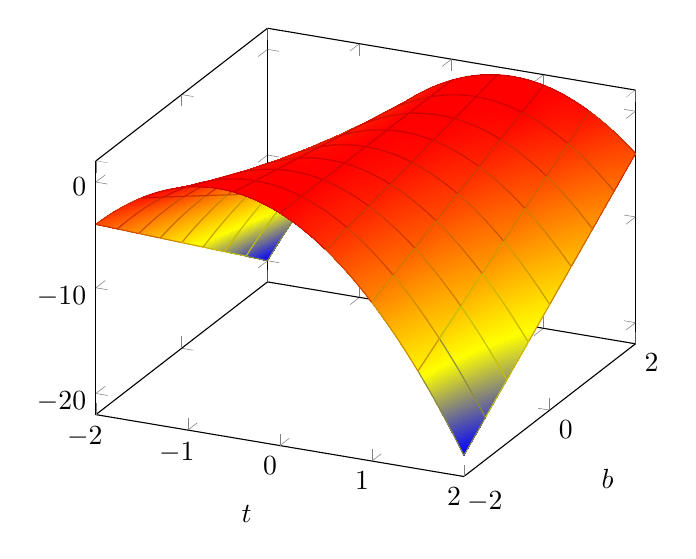
\begin{tikzpicture}
    \begin{axis} [xlabel = $t$, ylabel = $b$]
    \addplot3[patch,patch refines=3,
		shader=faceted interp,
		patch type=biquadratic] 
    table[z expr=-3*x^2 + 2*y*x]
    {
        t  b
        -2 -2
        2  -2
        2  2
        -2 2
        0  -2
        2  0
        0  2
        -2 0
        0  0
    };
    \end{axis}
\end{tikzpicture}
\caption{Gr\'afico de $f(b,t) = -3t^2 + 2bt$}
\label{fig:exercice_01_a_01}
\end{figure}

	Aceleraci\'on:

	$$ \frac{dv}{dt} = \frac{d(-3kt^2 + 2bt)}{dt} $$
	$$ a = -6kt + 2b $$

	Gr\'afico de la aceleraci\'on en funci\'on del tiempo, con $k=1$

	%h (here), le decimos que ponga la imagen m\'as o menos aqu\'i
%t (top), preferiblemente en la parte superior de la p\'agina
%b (bottom), preferiblemente en la parte inferior de la p\'agina
%p (page), que junte los objetos flotantes en una p\'agina
%! que ignore sus reglas internas de posicionamiento
%H que ponga la imagen justo aqu\'i, similar a h!
\begin{figure}[h]
\centering
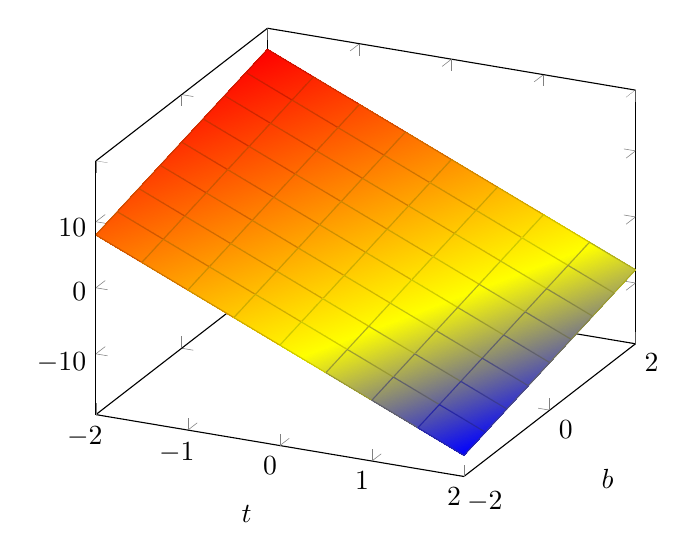
\begin{tikzpicture}
    \begin{axis} [xlabel = $t$, ylabel = $b$]
    \addplot3[patch,patch refines=3,
		shader=faceted interp,
		patch type=biquadratic] 
    table[z expr=-6*x + 2*y]
    {
        t  b
        -2 -2
        2  -2
        2  2
        -2 2
        0  -2
        2  0
        0  2
        -2 0
        0  0
    };
    \end{axis}
\end{tikzpicture}
\caption{Gr\'afico de $f(b,t) = -6t + 2b$}
\label{fig:exercice_01_a_01}
\end{figure}

\item

	Si $v = 0$ entonces
	
	$$ -3kt^2 + 2bt = 0$$
	
	Aplicando la \emph{f\'ormula de Bhaskara} (de ahora en m\'as \emph{resolvente}), nos queda
	
	$$ t_1, t_2 = \frac{-2b \pm 2b}{-6k} $$
	
	Es decir,
	
	$$ t_1 = 0$$
	$$ t_2 = \frac{2}{3} \frac{b}{k}$$
	
	Ahora podemos encontrar la respectiva posici\'on:
	
	$$ x(t_1) = 0 $$
	$$ x(t_2) = -k \frac{2b}{3k}^3 + b\frac{2b}{3k}^2 = \frac{4b^3}{27k^2}$$
	
\item

	Con $k = 0$, la aceleraci\'on sera siempre 0 o positiva. \\
	Con $b = 0$, la aceleraci\'on sera siempre 0 o negativa. \\
	Con $t < 0$ la aceleraci\'on sera siempre 0 o positiva. \\
	Con $t = 0$ la aceleraci\'on es 0.

\end{enumerate}
	\item \begin{enumerate}

\item

	Velocidad en funci\'on del tiempo:

	$$ v = \dv{x}{t} = \dv{\sqrt{x_0^2+2kt}}{t} $$
	$$ v = \frac{1}{2}\frac{2k}{\sqrt{x_0^2+2kt} }$$
	$$ v(t) = \frac{k}{\sqrt{x_0^2+2kt}} $$
	
	Aceleraci\'on en funci\'on del tiempo:
	
	$$ a = \dv{v}{t} = \dv{\frac{k}{\sqrt{x_0^2+2kt}}}{t} $$
	$$ a = \frac{0 - \frac{k^2}{\sqrt{x_0^2+2kt}}}{x_0^2+2kt} $$
	$$ a(t) = -\frac{k^2}{(x_0^2+2kt)^\frac{3}{2}} $$
	
\item
	
	En $t = 0$, dado que $x_0 > 0$, es v\'alido lo siguiente:
	$$ x(t = 0) = \sqrt{x_0^2} = \left| x_0 \right| = x_0 $$
	
	Velocidad:
	
	$$ v(x) = \frac{k}{x}$$
	
	Aceleraci\'on:
	
	$$ a(x) = -\frac{k^2}{x^3}$$
	
	Los gr\'aficos aproximados deben de ser tendiendo a cero mientras mas grande es el valor de $x$ y tendiendo a $\inf$ cuando el valor este m\'as pr\'oximo del $0$. La velocidad siempre ser\'a positiva y la aceleraci\'on negativa. 

\end{enumerate}
	\item \begin{enumerate}

\item

	Buscamos $x(t)$:
	
	$$ a = \dv{v}{t} = kt^2 $$
	$$ \dv{v}{t} = kt^2 $$
	$$ dv = kt^2 dt $$
	$$ \int \! \, dv = \int \! kt^2 \, dt $$
	$$ v + c_1 = \frac{kt^3}{3} + c_2 $$
	
	Con $c_2 - c_1 = c_3$, y adem\'as, sabiendo que $v(t_0) = v_0$, entonces $v_0 = 0 + c_3$, entonces $c_3 = v_0$. Nos queda:
	
	$$ v = \frac{kt^3}{3} + v_0 $$
	$$ \dv{x}{t} = \frac{kt^3}{3} + v_0 $$
	$$ dx = \frac{kt^3}{3} + v_0 dt $$
	$$ \int \! \, dx = \int \! \frac{kt^3}{3} + v_0 \, dt $$
	$$ x + c_4 = \frac{kt^4}{12} + v_0t + c_5$$
	
	Con $c_5 - c_4 = c_6$, y adem\'as, sabiendo que $x(t_0) = 0$, entonces $0 = 0 + c_6$, y se tiene $c_6 = 0$. Nos queda:
	
	$$ x = \frac{kt^4}{12} + v_0t$$
	
	Buscamos $x(v)$. Para esto, $x$ no debe depender del $t$, dado que sino depender\'ia de dos variables ($x(v,t)$). Entonces:
	
	$$ x = \left(\frac{kt^3}{12} + v_0 \right)t $$
	
	Pero adem\'as, de la velocidad tenemos que:
	
	$$ t = \sqrt[3]{\left( v - v_0 \right)\frac{3}{k}} $$
	
	Entonces
	
	$$ x = \frac{v - 3v_0}{4} \sqrt[3]{\left( v - v_0 \right)\frac{3}{k}} $$

\item

	Buscamos $x(t)$:
	
	$$ a = \dv{v}{t} = -kv^2 $$
	
	Pero si lo dejamos as\'i, agregar\'iamos la variable $t$, y esto es agregar informaci\'on innecesaria. Entonces:
	
	$$ a = \dv{v}{t} = -k\dv{x}{t}v $$
	$$ dv = -kvdx $$
	$$ \frac{1}{v}dv = -kdx $$
	$$ \int \! \frac{1}{v} \, dv = - \int \! k \, dx $$
	$$ \ln\left| v \right| + c_1 = -kx + c_2 $$
	
	Con $c_2 - c_1 = c_3$:
	
	$$ \ln\left| v \right| = -kx + c_3 $$

	Como el intervalo analizado es positivo para $v(t)$ (por $t > 0$),	
	
	$$ \ln v = -kx + c_3 $$
	$$ v = e^{-kx + c_3} $$
	
	Por las condiciones iniciales (en lo que sigue, \emph{CI}), $ v(t = 0) = e^{-kx(t = 0) + c_3} $ y entonces
	$ v_0 = e^{c_3} $. Despejando se tiene $c_3 = \ln v_0 $. Entonces
	
	$$ v = e^{-kx + \ln v_0 } $$
	$$ \dv{x}{t} = e^{-kx + \ln v_0 } $$
	$$ dx = e^{-kx + \ln v_0 }dt $$
	$$ e^{kx} dx = e^{\ln v_0 }dt $$
	$$ e^{kx} dx = v_0 dt $$
	$$ \int \! e^{kx} \, dx = \int \! v_0 \, dt $$
	$$ \frac{1}{k}e^{kx} + c_4 = v_0t + c_5 $$
	$$ e^{kx} = v_0kt + \left(c_5 - c_4\right)k $$
	
	Con $\left(c_5 - c_4\right)k = c_6$, y adem\'as, sabiendo que $x(t_0) = 0$, entonces $c_6 = 1$. Nos queda:
	
	$$ e^{kx} = v_0kt + 1 $$
	$$ kx = \lnb{v_0kt + 1} $$
	$$ x(t) = \frac{1}{k} \lnb{v_0kt + 1} $$
	
	Buscamos $x(t)$. Anteriormente encontramos el siguiente resultado:
	
	$$ v = e^{-kx + \ln v_0 } $$
	$$ \ln v = -kx + \ln v_0 $$
	$$ \ln v_0 - \ln v = kx $$
	$$ x(v) = \frac{\lnb{\frac{v_0}{v}}}{k} $$
	
\item

	Buscamos $x(t)$. Procediendo de forma an\'aloga:
	
	$$ \dv{v}{t} = k\dv{x}{t}x $$
	$$ dv = kx dx $$
	$$ \int \! \, dv = \int \! kx \, dx $$
	$$ v + c_1 = \frac{kx^2}{2} + c_2 $$
	$$ v = \frac{kx^2}{2} + v_0 $$
	$$ \dv{x}{t} = \frac{kx^2}{2} + v_0 $$
	$$ dx = \frac{kx^2 + 2v_0}{2}dt$$

	Con $v_0 \neq 0$	
	
	$$ \frac{2}{kx^2 + 2v_0}dx = dt$$
	$$ \frac{2}{2v_0} \int \! \frac{1}{\frac{kx^2}{2v_0} + 1} \, dx = \int \! \, dt$$

	Haciendo el siguiente cambio de variables, con $u = \frac{\sqrt{k}x}{\sqrt{2v_0}}$, 
	entonces $du = \sqrt{\frac{k}{2v_0}}$. Dado que $du$ es constante, el c\'alculo se vuelve sencillo:
	
	$$ \frac{1}{v_0} \sqrt{\frac{2v_0}{k}} \int \! \frac{1}{u^2 + 1} \, du = t + c_3 $$
	$$ \sqrt{\frac{2}{kv_0}} \arctan u = t + c_3 $$
	
	Y a $t = 0$ nos queda $c_3 = 0$, entonces
	
	$$ \sqrt{\frac{2}{kv_0}} \arctan \frac{\sqrt{k}x}{\sqrt{2v_0}} = t + c_3 $$
	
	Despejando:
	
	$$ x(t) = \tan{\sqrt{\frac{kv_0}{2}}t}\sqrt{\frac{2v_0}{k}}$$
	
	Buscamos $x(v)$. Partiendo de lo ya obtenido anteriormente:
	
	$$ v = \frac{kx^2}{2} + v_0 $$
	$$ v - v_0 = \frac{kx^2}{2} $$
	$$ \frac{2\left(v - v_0\right)}{k} = x^2 $$
	$$ \pm \sqrt{\frac{2\left(v - v_0\right)}{k}} = x $$
	
	Dado que $x$ es siempre positiva:
	
	$$ x(v) = \sqrt{\frac{2\left(v - v_0\right)}{k}}$$

\end{enumerate}
\end{enumerate}

%\appendix
%\chapter{Tabla de integrales}
%\input{}

\bibliography{biblio}
\addcontentsline{toc}{chapter}{Bibliograf\'ia}
%Las opciones de estilo mencionadas en ISO 690-2 son las siguientes.
%abntex2-num.bst
%El resto son incompatibles.
\bibliographystyle{iso690}

\end{document}